\documentclass[byrevtex,amssymb,aps,pra,floatfix,letterpaper]{revtex4}
\usepackage{graphicx}
\usepackage{hyperref}
\bibliographystyle{apsrev}
\date{\today}
\pagestyle{plain}
\newcommand{\degree}[0]{$^\circ$}

\begin{document}

\title{Experiment 5: Phase diagram for a three-component system}

\date{\today}

\maketitle

\section{Introduction}

It is sometimes necessary to know the mutual solubilities of liquids in a two-phase system. For example, you may need to know how much water is dissolved in an organic liquid with which it is in contact, and also the amount of the organic compound that is in the aqueous phase. In this experiment you will consider a three-component mixture (1-butanol -- water -- acetic acid at 25 $^\textnormal{o}$C and barometric pressure) and construct the corresponding ternary phase diagram. Examples of experiments using this methodology are given in Refs. \cite{CLARKE,STEAD,PARK}.

\section{The phase rule}

Information regarding phase equilibria can be predicted by a simple rule (``Gibbs phase rule''):

\begin{equation}
f = c - p + 2
\label{eq1}
\end{equation}

\noindent
where $c$ is the number of components and $p$ is the number of phases present in the system. The degrees of freedom $f$, or variance, gives the number of variables (e.g., pressure, temperature, composition, etc.) that must be given to completely describe the system, or to locate the state of the system on the phase diagram.\\

\noindent
\textbf{Example.} For pure gas (e.g. one component system) $c = 1$ (pure gas; only one component) and $p = 1$ (only one phase; the gas phase) and by Eq. (\ref{eq1}) we have $f = 2$. This means that two variables are required for complete description of pure gas (i.e., any two of the three variables $P$, $V$ or $T$).\\

\noindent
\textbf{Example.} Consider water with the phase diagram shown in Fig. \ref{fig1}.

\begin{figure}[!htp]
\begin{center}
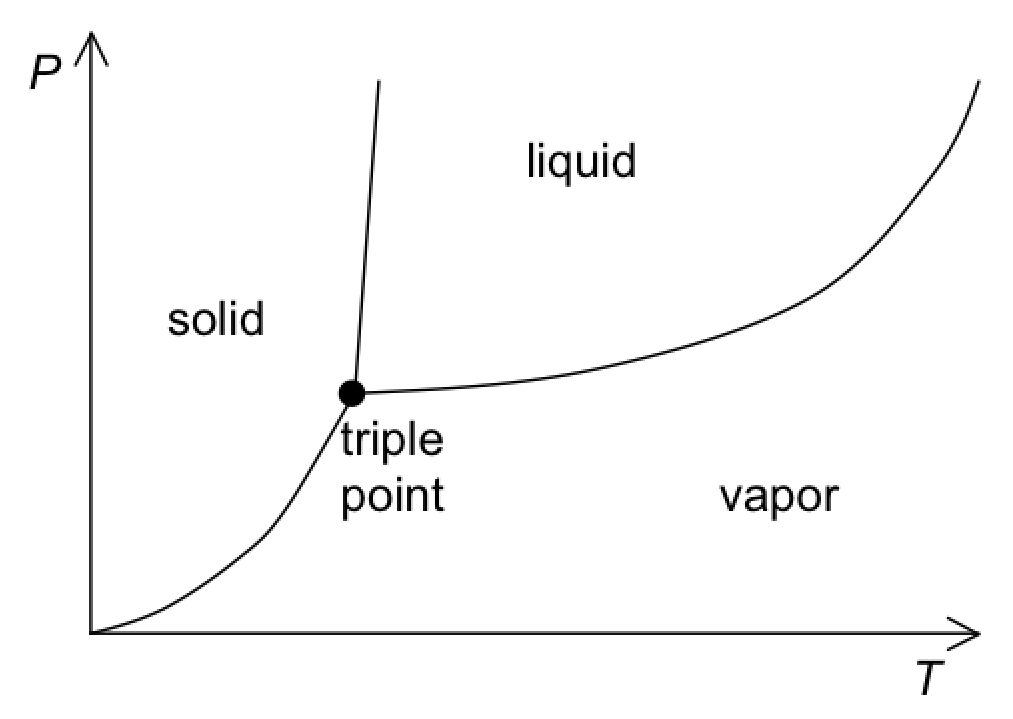
\includegraphics[scale=0.5]{fig1}
\caption{A schematic drawing of the phase diagram for water.}
\label{fig1}
\end{center}
\end{figure}

For pure phases (solid, liquid or vapor) $f = 2$. When two phases are present simultaneously (e.g. the point resides on the lines separating the phases in Fig. \ref{fig1}), only $P$ or $T$ can be varied independently and the phase rule gives $f = 1$. When all three phases are present (i.e., the triple point), all variables must be fixed and the phase rule says that $f = 0$.

For ternary systems (i.e., consisting of three components), we have $c = 3$ and $f = 5 - p$. If the system consists of only one phase, $f = 4$. The required four variables for describing such system are: two for describing the relative composition (mass fractions) and one of the pairs ($P$, $V$), ($P$, $T$), or ($T$, $V$). Note that if only two mass fractions $x_1$ and $x_2$, are given, the third can be obtained by $x_3 = 1 - x_2 - x_1$. Also in practice, ($P$, $T$) pair is chosen. If the system separates into two different phases, only $f = 5 - 2 = 3$ variables are needed (one mass fraction and ($P$, $T$)).

Phase diagrams for ternary systems are usually represented using a triangle shown in Fig. \ref{fig2}. This graph accounts for the fact that only two variables are required. Along the phase boundary only one variable is required.

\begin{figure}[!htp]
\begin{center}
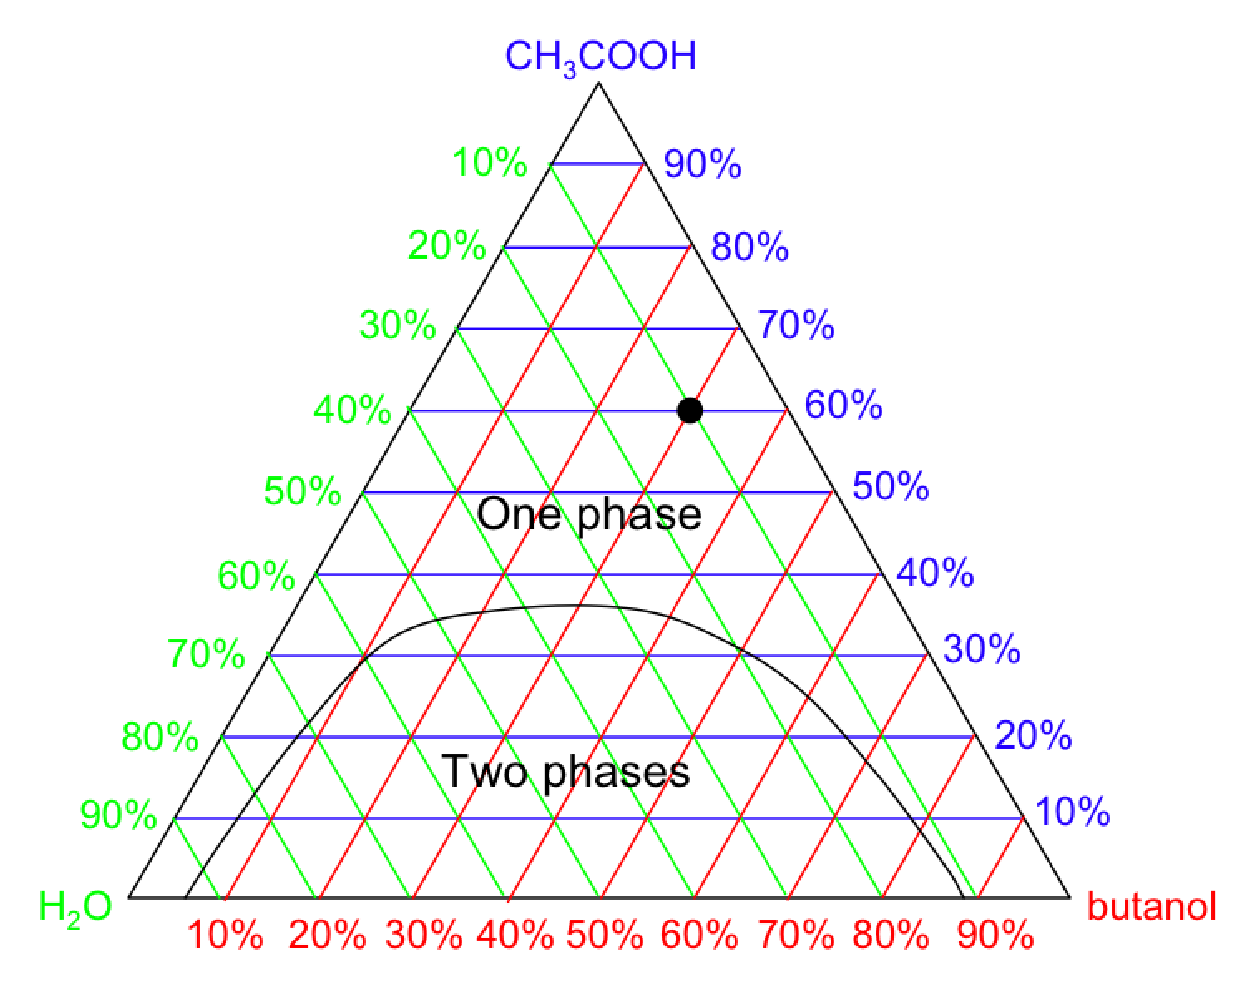
\includegraphics[scale=0.5]{fig2}
\caption{A triangular phase diagram showing the representation of the mass fractions for ternary systems. The colors indicate how concentrations for different species should be read from the diagram. The point marked in the diagram ($\bullet$) represents 30\% 1-butanol, 10\% water and 60\% acetic acid. The one- and two-phase regions have been separated by a black line. The line drawn is only demonstration and does not correspond to experimental observation. Pressure and temperature are assumed to be fixed.}
\label{fig2}
\end{center}
\end{figure}

Regions where one or two phases appear have also been indicated in Fig. \ref{fig3}. Note that the line drawn is hypothetical, the real curve will be determined in this experiment. When the solution is stirred, the transition from one region to another can be observed by appearance (or disappearance) of cloudiness or turbidity in the solution. The turbidity results from scattering of light by the large number of very small ``oily'' droplets of the second phase that are produced when the system is stirred. Sometimes it is easier to see this when stopping the stirring briefly.

If the three components are mixed to give an overall system composition that falls in the 2-phase region, the system will separate into two phases: a phase rich in water and another rich in 1-butanol. The compositions of the phases that form are given by the intersections of a tie line with the phase boundary. The tie line must also contain the point describing the overall system composition. A graphical demonstration and an interpretation of a tie line are given in Fig. \ref{fig3}.

\begin{figure}[!htp]
\begin{center}
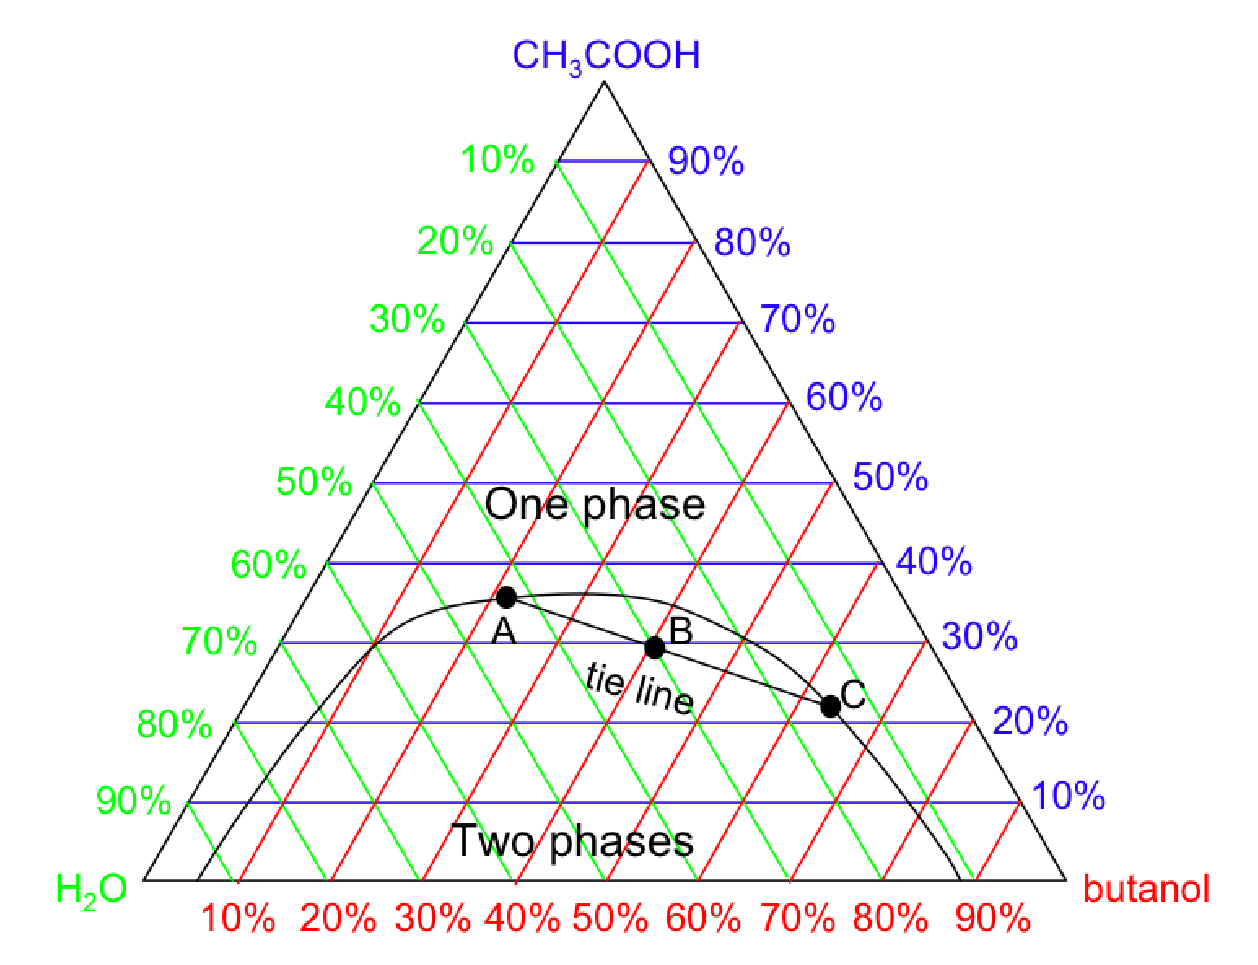
\includegraphics[scale=0.5]{fig3}
\caption{Drawing of a tie line in a triangular phase diagram. The diagram may contain one or many tie lines. The point 'A' denotes the composition of phase 1, 'B' denotes the initial composition of the system, and 'C' the composition of phase 2.}
\label{fig3}
\end{center}
\end{figure}

Note that in the case of Fig. \ref{fig3} only the mass fraction of 1-butanol must be given when the system remains on the phase boundary line. This determines the mass fractions for water and acetic acid. Hence the phase rule holds with $f = 5 - p = 3$ (i.e., mass fraction for 1-butanol,  temperature and pressure). If the system was initially in the two-phase region, the tie line uniquely connects the points along the phase separating line. Given the point 'A' in Fig. \ref{fig3} (depending on the 1-butanol mass fraction in phase 1), the points 'B' and 'C' are uniquely determined. Thus only the 1-butanol mass fraction in phase 1, temperature and pressure are required for complete description of the system, which had separated into two phases. This is again in accordance with the phase rule.

\section{Experimental}

\noindent
\underline{Task overview:} In the first part of the experiment, solubility of 1-butanol in water and solubility of water in 1-butanol will be determined. The switch to the two-phase region can be observed as appearance of the turbidity in the stirred solution. This gives the first two points in the phase diagram that lie along the horizontal axis (see Fig. \ref{fig2}; ``the starting points for the arc''). In the second part, the points defining the arc will be determined by
starting from the two-phase region and adding 17.5 M acetic acid (molecular weight 60.05 g mol$^{-1}$) until the system switches into one phase. This transition can be observed by disappearance of the turbidity in the stirred solution. In the third part one of the tie lines is determined experimentally. This will be done by choosing a point from the two-phase region and determining the compositions of the two phases formed.\\

\noindent
\underline{Part 1:}\\

\begin{enumerate}
\item Place 20 mL of water in a 50 mL Erlenmeyer flask. Cover the flask with Parafilm. Poke the buret containing 1-butanol through the Parafilm. Add 1-butanol to the water drop by drop with continuous stirring until the turbidity (``small oily droplets form''; this is difficult to see -- be careful!) appears and remains for at least 5 min. It will take less than 2 mL of 1-butanol to reach this point. Record the amount 1-butanol required.

\item Place 20 mL of 1-butanol in a 50 mL Parafilm-covered Erlenmeyer flask. Add water to the 1-butanol drop by drop with continuous stirring until the turbidity appears and remains for at least 5 min It will take more than 2 mL but less than 5 mL to reach this point. Record the amount of water required.

\end{enumerate}

\noindent
\underline{Part 2:}\\

\begin{enumerate}
\item Place 20 mL of 1-butanol and 5 ml of water in a 200 mL Parafilm-covered Erlenmeyer flask. Add acetic acid drop by drop while continuously stirring the solution until the turbidity disappears. Record the volume of acetic acid added.

\item Add an additional 5 mL aliquot of water to the mixture from the previous step. Again titrate the stirred solution with acetic acid until the turbidity disappears. Record the volume of acetic acid added.

\item Continue adding water in 5 mL aliquots and titrating to the turbid point with acetic acid until a total of 30 mL water has been added. After this add 10 mL aliquots and keep titrating until a total of 110 mL of water has been added. Record the volumes of acetic acid added at each stage.

\end{enumerate}

\noindent
\underline{Part 3:}\\

\noindent
Mix 25 mL of water and 25 mL of 1-butanol. Stir for 5 min and let the solution settle into two phases. Add 3 mL of acetic acid and stir again for 5 min and let the solution settle. Place the solution in a separating funnel and separate. Determine the mass of each phase. Titrate the bottom phase with standardized 1.0 M NaOH. Obtain an average of three runs. Use three drops of 1\% phenolphthalein solution as indicator (acidic = no color, basic = pink color, strongly basic = no color). Note that the standardization of NaOH must be done during the period that the bottom -phase titration is done since the NaOH concentration changes rapidly when carbon dioxide is absorbed from the atmosphere. Use 0.25 M solution of dried potassium hydrogen phthalate (KHP; M.W. 204.23 g mol$^{-1}$) for standardization. Use the same indicator for standardization.

\section{Data analysis}

Calculate mass fractions $x_i$ (in \%) for each component in every solution (i.e., parts 1 and 2 in previous section) using the following equation:

\begin{equation}
x_i = \frac{V_i\rho_i}{\sum\limits_{i=1}^3V_i\rho_i}\times 100\%
\label{eq2}
\end{equation}

\noindent
where $V_i$ is the volume and $\rho_i$ the density of the component $i$ (water, acetic acid, 1-butanol).  The densities of water, 1-butanol and acetic acid are 0.9970, 0.8098 and 1.046 kg L$^{-1}$, respectively. Plot the phase boundary data on the triangular paper given at the end of this document. From the results obtained in part 3, determine the weight percent of the three components in each phase. Note that in part 3 just by knowing the mass percentage of acetic acid allows you to determine the 1-butanol and water concentrations as well (use the phase diagram previously determined and note that the points in part 3 must land on the phase boundary arc). However, there are two possibilities (i.e., the acetic acid mass fraction line can intersect the phase boundary arc at two different points) but you know that the densest liquid will reside in the bottom phase and this allows you to discard one of the points. The same applies for the top phase. The mass fraction for the top phase can be calculated as: ``the total amount of acetic acid'' -- ``the amount of acetic acid in the bottom phase''. Put the previously calculated two points on the triangular graph along with a point for the initial composition and draw the tie line between the three points.

\section{Written laboratory report}

Follow the general instructions for written laboratory reports. In addition, include the requested data in the following section:\\

\noindent
\textit{Results.} This section should include the triangular phase diagram along with numerical data.\\

\noindent
\textit{Questions \& Answers.} Prepare answers to the following questions (length: $<$ 3):\\

\begin{enumerate}
\item For the two solutions with no acetic acid calculate the mole fraction of water and 1-butanol in each. Give a qualitative explanation why 1-butanol is rather insoluble in water while water is rather soluble in 1-butanol. Identify the interactions that are important for solvation processes.
\item If two moles of water and one mole of 1-butanol are mixed, will two phases result? If so, what will be the mole fractions of water and 1-butanol in each phase? Which has a lower free energy, a single-phase or two-phase solution in this case?
\item If two moles of 1-butanol and one mole of water are mixed, will two phases result? If so, what will be the mole fractions of water and 1-butanol in each phase? Which has a lower free energy, a single-phase or two-phase solution in this case?
\item Give a \textit{qualitative} explanation why addition of acetic acid makes the two-phase mixture of 1-butanol and water into a one-phase system?
\item Determine $c$ (the number of components), $p$ (the number of phases) and $f$ (the variance) of the system in each region of the phase diagram.
\end{enumerate}

\section{References}

\vspace{-1cm}

\bibliography{../references}

\newpage
\begin{figure}[!htp]
\begin{center}
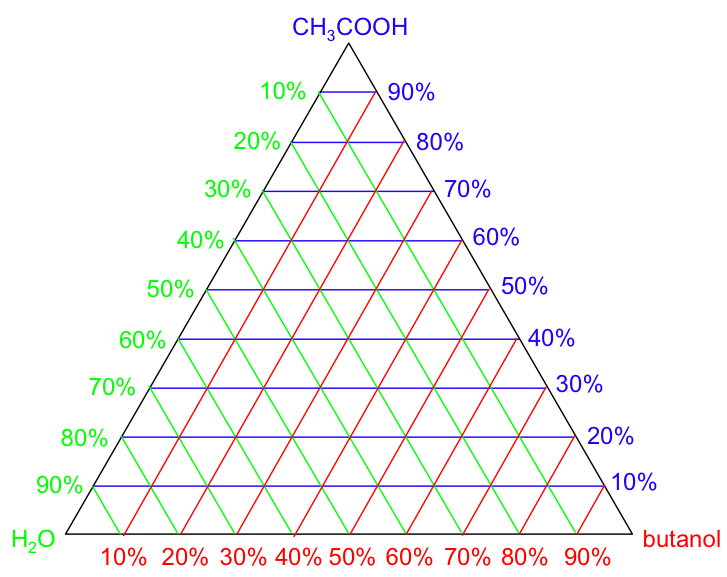
\includegraphics[scale=0.8]{fig4}
\caption{Triangular phase diagram template}
\label{fig4}
\end{center}
\end{figure}

\end{document}
